\begin{figure}[h!]
	\centering
	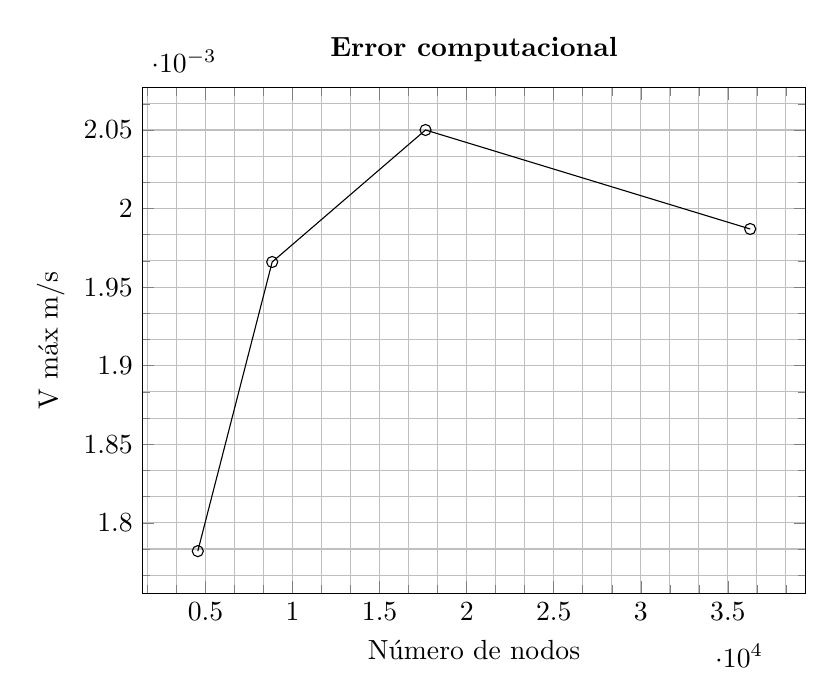
\begin{tikzpicture}
		\begin{axis}[
			grid = both, minor tick num=2,
			title = \textbf{Error computacional},
			xlabel = N\'umero de nodos,
			ylabel = V m\'ax m/s,
			legend pos = outer north east,
			width=10cm, height=8cm
		]
		%\addplot[blue, line width=2pt] {\val};
		\addplot[
        scatter,scatter src=explicit symbolic,
        scatter/classes={
            a={mark=o,black},
            b={mark=triangle*,red},
            c={mark=o,draw=black,fill=black}
        }
    ]
    table[x=x,y=y,meta=label]{
        x	y	label
		4560	0.001782	a
		8832	0.001966	a
		17636	0.002050	a
		36280	0.001987	a
    };
		%\legend{Te\'orico, Num\'erico};
		\end{axis}
	\end{tikzpicture}
	\caption{Cambio de la velocidad m\'axima con respecto al refinamiento de malla.}
	\label{resumErrG}
	\end{figure}